%!TEX root = ../Physik I.tex

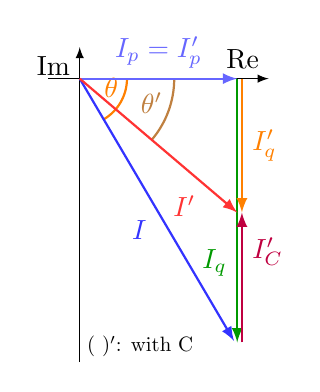
\begin{tikzpicture}[>=latex,scale=2]
	\begin{scope}
		\draw[->] (0,-1.8) -- (0,.2) node[below left]{Im};
		\draw[->] (-.2,0) -- (1.2,0) node[above left]{Re};
	\end{scope}
	
	\begin{scope}[thick]
		\draw[color=orange] (.3,0) arc (0:-60:.3cm) node[above, yshift=.15cm, xshift=.1cm]{$\theta$};
		\draw[color=brown] (.6,0) arc (0:-40.5:.6cm) node[above, yshift=.2cm]{$\theta'$};
		\draw[->,color=blue!80,scale=.98] (0,0) -- (1,-1.7) node[pos=.5,below left]{$I$};
		\draw[->,color=green!60!black] (1,0) -- (1,-1.675) node[pos=.7,left]{$I_q$};
		\draw[->,color=blue!60] (0,0) -- (1,0) node[pos=.5,above]{$I_p = I_p'$};

		\draw[->,color=red!80] (0,0) -- (1,-.85) node[pos=.8,below left]{$I'$};
		\draw[->,color=orange,xshift=.03cm] (1,0) -- (1,-.85) node[pos=.5,right]{$I_q'$};
		\draw[->,color=purple,xshift=.03cm] (1,-1.675) -- (1,-.85) node[pos=.7,right]{$I_C'$};
	\end{scope}
	
	\begin{scope}
		\draw (0,-1.7) node[right,scale=.75] {$(\ )'$: with C};
	\end{scope}
\end{tikzpicture}